%#!platex main

\chapter{字句解析}
\label{103559_30Mar06}

\section{用語}

説明を始める前に、この章を通して用いられる用語を整理しておくことにしよう。

\ref{134201_29Mar06}節で述べたように、字句解析の目的は、文字列としての原
始プログラムから意味のある文字列を切り出すことである。ここで言う「(原始
言語で)意味のある文字列」のことを{\bfseries 字句要素}(lexeme)という。
例えば、C言語の字句要素には次のようなものがある。
\begin{itemize}
 \item 変数名、関数名などの{\bfseries 識別子}(identifier)
 \item \icode{int}, \icode{while}など、C言語プログラム中で特別な意味を持
       ち、他の用途に用いることのできない語({\bfseries 予約語}, keyword)
 \item データの値を表す{\bfseries 定数}(constant)。整数定数、浮動小数点
       定数、文字定数などがある。
 \item 文字列を表す{\bfseries 文字列リテラル}(string literal)
 \item \icode{+}, \icode{*}, \icode{=}, \icode{==}などの{\bfseries 演算
       子}(operator)
 \item 括弧、セミコロンなどの{\bfseries 区切り記号}(separator)
\end{itemize}
空白、タブ、改行文字、コメントなどはC言語のプログラムの意味には影響を与え
ないので、字句解析の際に捨てられる。

実際の字句解析では、切り出した字句要素をそのまま構文解析部に渡すことはせ
ず、字句要素を{\bfseries トークン}(token)というデータに変換してから渡す。
トークンには以下のような情報が含まれる。
\begin{itemize}
 \item 字句要素の種類。例えば\icode{ID}(識別子)、\icode{IF}(予約語
       \icode{if})、\icode{RELOP}(比較演算子)など\footnote{以降、特に
       断らない限り、英大文字と数字からなるゴシック文字列を字句要素の種類
       として用いる。}。
 \item 付加情報。例えば、識別子\icode{argc}には、その識別子の名前、すなわ
       ち ``argc'' が付加情報として付けられる。また整数定数 \icode{453}
       には、その定数の値、すなわち 453 という整数が付加情報として付けら
       れる。付加情報のない場合もある。
\end{itemize}

\section{素朴な字句解析とその問題点}
\label{170323_24Apr06}

字句解析アルゴリズムの前提として、原始プログラムを読む回数は1回に押さえた
い。つまり、原始プログラムのファイルを初めから終わりまで順に1回読み込むだ
けで字句解析を終わらせるようにしたい。これは、CPUの計算に比べて、ファイル
(二次記憶)との入出力はずっと時間がかかるからである。

また、コンパイラ中に巨大な文字配列を確保し、そこに原始プログラムを全部読
み込んでから字句解析をするという方法も好ましくない。巨大な配列を確保する
と、コンパイラの使用メモリ量が増えてしまう。コンパイラは比較的重いプログ
ラムなので、なるべく使用メモリ量を節約して設計したい。

すると、素朴な字句解析プログラムは次のようになるであろう。原始プログラム
ファイルから\icode{getc()}関数で1文字読み、その種類によって場合分けを
行う。これをファイルの終わりまで繰り返す。

\begin{quote}
\begin{lstlisting}[language=C]
 #include <stdio.h>
 /* 後述するように、字句要素は整数で表現する */
 #define IF 1
 /* 以下、字句要素の定義が続く */

 /* 次の字句要素の番号を返す */
 int simple_lexical_analysis()
 {
   char c;
   /* file: 原始プログラムファイル */
   while((c = getc(file)) != EOF) {
     /* 予約語 if の処理 */
     if (c == 'i') {
       c = getc(file);
       if (c == 'f') {
         return IF;
       }
     }
     /* 以下、他の字句要素の処理が続く */
   }
 }
\end{lstlisting}
\end{quote}

しかし、このプログラムには問題がある。字句要素ごとの処理が複雑になってし
まうのである。C言語には、iで始まる予約語は\icode{if}の他に\icode{int}もあ
る。またユーザが i で始まる識別子を使う可能性も高い。このような可能性をす
べて網羅して場合分けを書くのは大変である。ましてやこのプログラムを自動的
に生成するのは難しい。

以下の節では、正則表現を用いて字句解析部を自動的に生成する手法を述べる。

\section{正則表現を基にした字句解析}
\label{112953_24Apr06}

\begin{figure}
 \begin{center}
  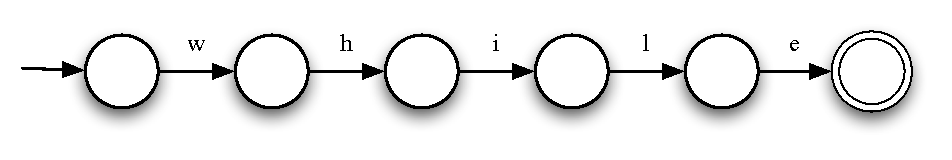
\includegraphics[width=13cm]{figure/fa_while.pdf}
 \end{center}
 \caption{\icode{while}に対応する有限オートマトン}
 \label{163948_18Apr06}
\end{figure}
\begin{figure}
 \begin{center}
  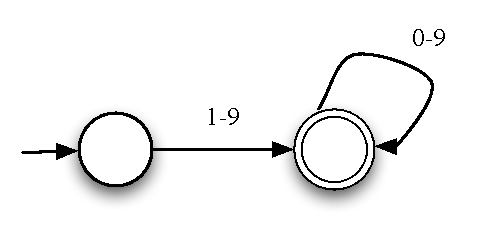
\includegraphics{figure/fa_decimal.pdf}
 \end{center}
 \caption{10進数に対応する有限オートマトン}
 \label{164232_18Apr06}
\end{figure}

字句解析の手法では、次のことを考える必要がある。
\begin{enumerate}
 \item 字句要素を定義する方法
       \label{075512_23Apr08}
 \item \ref{075512_23Apr08} で定義した字句要素を検出する方法
       \label{075846_23Apr08}
 \item 字句要素を検出したときに何らかの動作を行う方法(整数定数の字句要
       素を検出したときにその整数の値を求める、など)
\end{enumerate}

ここで述べる字句解析手法では、各字句要素を正則表現で表し、対応する有限オートマトン
を構成して字句要素を受理させる。上に述べた\ref{075512_23Apr08} の実現方法
として正則表現を、\ref{075846_23Apr08} の実現方法として有限オートマトン
を利用するのである。例えば、予約語
\icode{while}に対応する正則表現は$while$であり、この正則表現と等価な有限
オートマトンは図\ref{163948_18Apr06}のようになる。また、C言語の10進定数は
0以外の数字から始まる数字の列であるので、これに対応する正則表現は
$[1\mbox{-}9][0\mbox{-}9]^\ast$であり、これと等価な有限オートマトンは図
\ref{164232_18Apr06}のようになる。

このような有限オートマトンをすべての字句要素に対して作り、並列に動作させ
る。つまり、原始プログラムファイルから1文字読み込んで、それを入力記号とし
てすべての有限オートマトンを動作させる。これを繰り返して、ある有限オート
マトンが受理状態に到達すれば、字句要素が見つかったことになる。例えば
`w', `h', `i', `l', `e' の順に原始プログラムファイルから文字を読み込んだ
とすると、図\ref{163948_18Apr06}の有限オートマトンは受理状態に到達し、一
方、それ以外の有限オートマトン(例えば図\ref{164232_18Apr06}のオートマト
ン)は受理状態に到達しない。従って、字句要素\icode{while}が見つかったこと
になる。字句要素が1つ見つかれば、すべての有限オートマトンをリセットし(初
期状態に戻して)、再び原始プログラムファイルからの文字の読込みを始める。

ただし、この方法ではまだ問題点が残っている。
\begin{figure}
 \begin{center}
  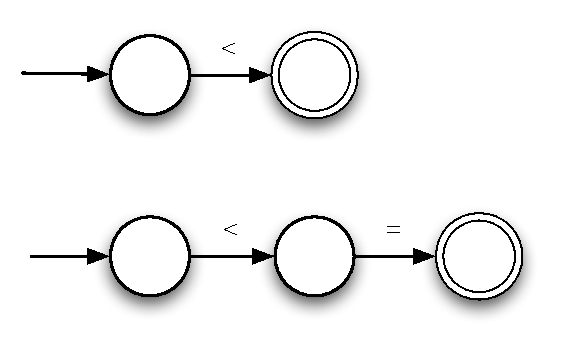
\includegraphics{figure/fa_relop.pdf}
 \end{center}
 \caption{比較演算子に対する有限オートマトン}
 \label{182549_18Apr06}
\end{figure}
\begin{figure}
 \begin{center}
  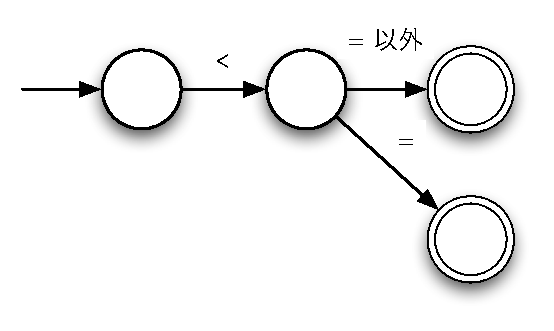
\includegraphics{figure/fa_relop_fixed.pdf}
 \end{center}
 \caption{比較演算子に対する有限オートマトン(改良版)}
 \label{183745_18Apr06}
\end{figure}
\begin{figure}
 \begin{center}
  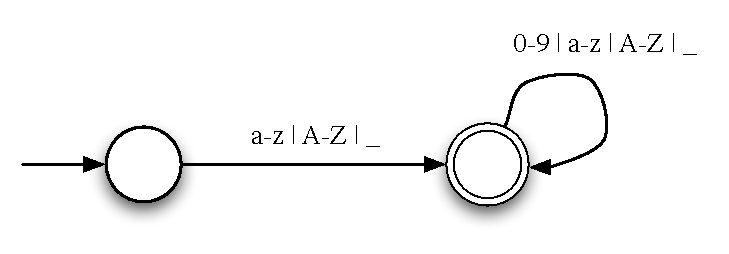
\includegraphics{figure/fa_identifier.pdf}
 \end{center}
 \caption{識別子に対する有限オートマトン}
 \label{081246_19Apr06}
\end{figure}
\begin{enumerate}
 \item 一つの文字列が2つ以上の有限オートマトンで受理されることがある。例
       えば文字列 `while' は図\ref{163948_18Apr06}の有限オートマトンで受
       理されるが、C言語の識別子を受理する有限オートマトン(図
       \ref{081246_19Apr06}、練習問題\ref{ex:regexp_05}を参照)でも受理さ
       れる。この場合、C言語では予約語として解釈しなければならない。すな
       わち、図\ref{163948_18Apr06}の有限オートマトンを優先して処理しなけ
       ればならない。
 \item (最長一致の原則) 字句要素を認識するときは、最も長いものを採用しな
       ければならない。例えば\verb|<|と\verb|<=|という2つの字句要素を考え
       よう。これらの字句要素を受理する有限オートマトンを図
       \ref{182549_18Apr06}に示す。`\verb|<|'を読み込んだとき、上のオート
       マトンは受理状態に到達する。しかし、もしこの次の文字が `\verb|=|'
       であれば、\verb|<|ではなく\verb|<=|という字句要素と解釈しなければ
       ならない。つまり、下のオートマトンのみで受理させなければならない。
       \label{183630_18Apr06}
\end{enumerate}

\ref{183630_18Apr06}に挙げた図\ref{182549_18Apr06}の問題点を改良する一つ
の案を図\ref{183745_18Apr06}に示す。ポイントは、`\verb|<|'を受理する有限オー
トマトンを改良し、`\verb|<|'の次に `=' 以外の文字を読み込んだときに受理す
る、とした点である。一般に、最長一致の原則はこれと同様の方法で解決できる。

ただし、注意しなければならない点がある。上のオートマトンで字句要素
`\verb|<|'を受理したとき、本来の字句要素`\verb|<|'よりも1文字余計に読み込
んでしまっている。この余計に読み込んだ文字は、次の字句要素を構成する文字
であるかもしれないため、`\verb|<|'を受理した後、読み込みを破棄しておかな
ければならない。

\section{字句解析プログラムの実現}
\label{170501_24Apr06}

\begin{figure}
 \begin{center}
  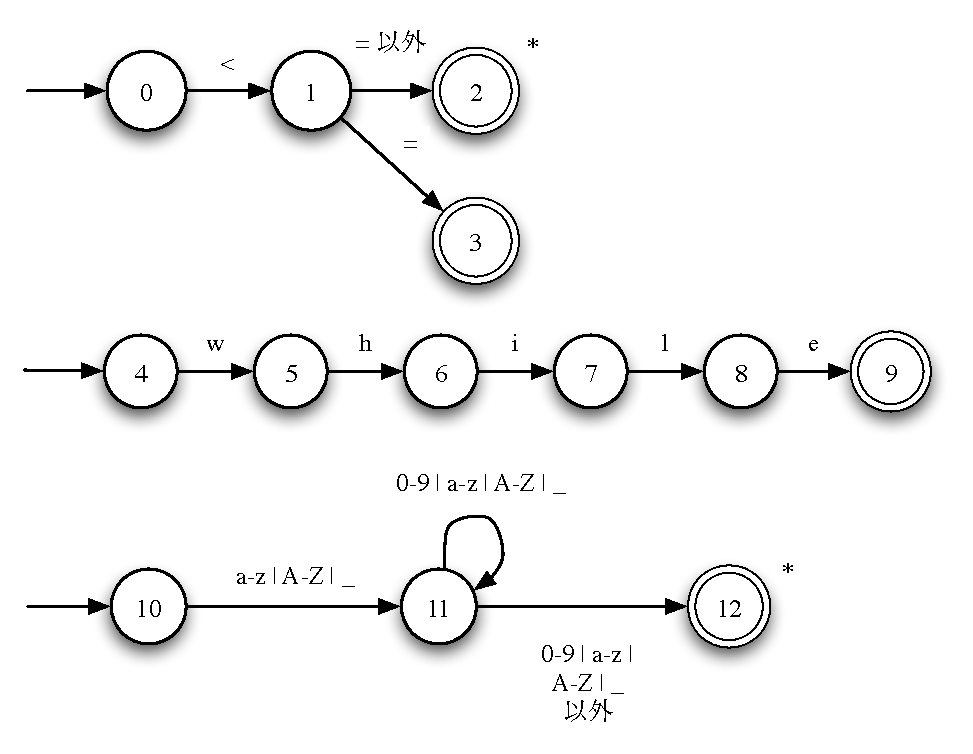
\includegraphics[width=13cm]{figure/lexical_analysis_example.pdf}
 \end{center}
 \caption{字句解析のための有限オートマトン群}
 \label{112450_24Apr06}
\end{figure}

有限オートマトンを基礎とする字句解析プログラムの実現について説明を行う。
なお、説明のため、ここでは認識すべきトークンを\verb|<|, \verb|<=|,
\icode{while}, それにC言語の識別子のみとする。また、これらのトークンを認
識する有限オートマトンの状態に番号を付けておく(図\ref{112450_24Apr06})。

\subsection{ファイルとの入出力}

これから作成する字句解析プログラムは、原始プログラムファイルから1文字ずつ
文字を読み、処理する、という操作をファイルの終わりまで繰り返す。ただし、
\ref{112953_24Apr06}節で述べたように、字句によっては、字句を認識した後に読
み込みを破棄しておかなければならない。

したがって、原始プログラムファイルからの読み込みは\icode{getc()}関数を、
読み込みの破棄は\icode{ungetc()}関数をそれぞれ用いればよい
\footnote{\icode{ungetc()}関数は今まで使ったことがないと思われるので、オ
ンラインマニュアルなどでどういう関数か調べておくこと。\icode{getc()}関数
を知らない、もしくは忘れている場合もオンラインマニュアルなどで調べておく
こと。}。ただし、この部分は後で改良を試みたいので、直接\icode{getc()},
\icode{ungetc()}を使うのではなく、次のような関数を通して使うことにする。

\begin{lstlisting}
 int nextchar(FILE* infile)
 {
    return getc(infile);
 }

 void backchar(int c, FILE* infile)
 {
    ungetc(c, infile);
 }
\end{lstlisting}

\subsection{データの表現}

コンパイラでは通常、原始言語のトークンに通し番号を付け、コンパイラの内部
でもその番号(整数)でそれぞれのトークンを表す。次の例では、
\verb|<|, \verb|<=|, \icode{while}, 識別子にそれぞれ 0, 1, 2, 3 という番
号を割り当てている。

\begin{lstlisting}
 #define LT  0
 #define LE  1
 #define WHILE 2
 #define ID  3
\end{lstlisting}

すると次節で示すように、字句解析プログラムはトークンを表す番号を返り値と
する関数となり、したがって\icode{int}型の値を返す関数となる。

ただし識別子については、実際の識別子名(\icode{i}, \icode{main}などの変数
名や関数名)も字句解析の出力とする必要がある。これは大域変数\icode{char~%
yytext[80];}に格納されるものとする\footnote{字句解析部の後に続く構文解析
部から識別子名を参照できるように、大域変数を用いている。}。

字句解析プログラムでは、ほかに次のような大域変数を用いる。
\begin{itemize}
 \item \icode{int state;}…有限オートマトンの現在の状態を表す。初期値は0。
 \item \icode{int initial\_state;}…現在処理中の有限オートマトンの初期状態
       を表す。初期値は0。
 \item \icode{FILE *file;}…原始プログラムのファイルポインタ。
\end{itemize}

\subsection{字句解析プログラム}

次に、字句解析プログラムの本体である\icode{nexttoken()}関数のコードを示す。
この関数は、構文解析部から必要に応じて呼び出されることを想定しており、次
のトークンを表す番号を返り値とする。また、トークンが識別子の場合には、大
域変数\icode{yytext}にその識別子名を格納する。

\begin{quote}
 \lstinputlisting[numbers=left]{code/nexttoken.c}
\end{quote}

大まかには、現在の状態(\icode{state})と次の文字(\icode{c})から次の状
態を決定し、\icode{state}の値を更新し、状態による分岐を行う(35行目)。そ
の結果受理状態に到達すれば、認識したトークンの番号を返す。受理状態に到達
できなかった場合は、\icode{fail()}関数を呼び出し、初期状態\icode{start}の
値を更新して次のオートマトンによる受理を試す。これをオートマトンの数だけ
繰り返していく。どのオートマトンでも受理できなかった場合は、原始プログラ
ムに誤りがあったことになるので、エラー処理を行う
\footnote{\icode{isalpha(c)}関数、\icode{isdigit(c)}関数はそれぞれ、
\icode{c}がアルファベットか、\icode{c}が数字かを判定する関数である。詳細
はオンラインマニュアルなどを参照のこと。}。

図\ref{112450_24Apr06}で$\ast$を付けた状態は、認識したトークンよりも1文字
先まで読み込んでしまっていることを示す。例えばトークン `\verb|<|'は、トー
クンの読み込み自体は状態1で終了しているが、`\verb|<|'か`\verb|<=|'かを決
定するために1文字先まで読み込み、状態2に至る必要がある。識別子も、識別子
に含まれない文字が出てきた時点で初めて、識別子の終わりが認識できるため、
状態12 に到達したときには1文字先まで読んでしまっていることになる。そのた
め、状態2と状態12については、\icode{backchar()}関数により、1文字分読み込
みを破棄している。

入力の破棄はオートマトンを切り替える際にも発生する。例えば状態6で、文字
`a'を読み込んでトークン\icode{while}の認識に失敗した場合、すでに読み込ん
だ `w', `h', `a'を破棄してから次のオートマトンに切り替えなければならない。
そのために、既に読み込んだ文字を蓄える配列\icode{s}、読み込んだ文字数を保
持する変数\icode{i}を局所変数として用意している。\icode{fail()}を呼び出す
ときには\icode{s}と\icode{i}を引数として渡し、\icode{fail()}中で入力の破
棄を行っている。

また状態12では、現在の\icode{s}の内容、すなわち認識した識別子名を大域変数
\icode{yytext}にコピーしている。

\subsection{字句解析部自動生成プログラム\icode{lex}}

\ref{170501_24Apr06}節で示した字句解析プログラムは各状態で行うべき処理が
かなりパターン化されており、図\ref{112450_24Apr06}のオートマトンが与えら
れれば、\ref{170323_24Apr06}節で示したプログラムに比べて自動的に生成しや
すい。

実は、字句解析部を自動生成するプログラムはいくつもある。これらはいずれも、
認識すべきトークンの正則表現と、トークンに対して行うべき処理を指定すると、
字句解析プログラムを自動生成してくれる。内部的には、正則表現から図
\ref{112450_24Apr06}に相当するオートマトンを自動生成し(アルゴリズムは例
えば\cite{ホップクロフト03:automaton}を参照)、さらに
\ref{170501_24Apr06}節に示したような字句解析プログラムを自動生成している。

例として、Unixに標準装備されている\icode{lex}プログラムを取り上げる。
\ref{170501_24Apr06}節のプログラムと同等の字句解析プログラムを自動生成す
るには、以下のようなルールを書き、\icode{lex}で処理すればよい。

\begin{quote}
 \lstinputlisting{code/nexttoken.lex}
\end{quote}

`\verb|%{|'から `\verb|%}|'までがトークンの番号指定、`\verb|%%|'に挟まれ
た部分が認識すべきトークンを表す正則表現と、そのときに行われる処理(C言語
プログラム)である。識別子名は自動的に\icode{yytext}という変数に格納され
る。

\icode{lex}やその他の字句解析部自動生成ソフトウェアの詳細は、ここでは省略
する。各自で適宜参考資料にあたられたい。

\section{入力のバッファリング}

本章の最後に、\icode{nextchar()}関数、\icode{backchar()}関数の改良につい
て考えよう。

\begin{figure}
 \begin{center}
  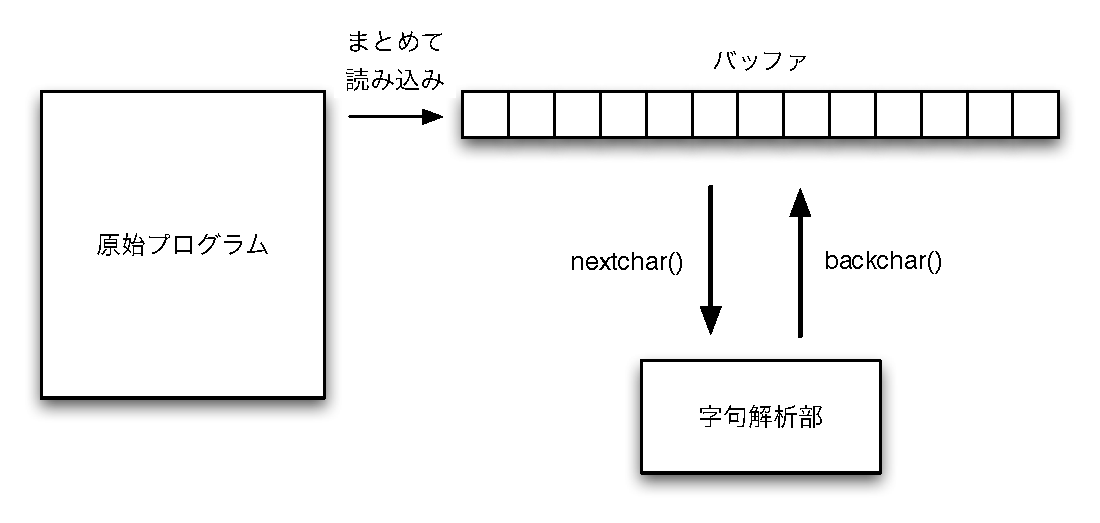
\includegraphics[width=13cm]{figure/buffering.pdf}
 \end{center}
 \caption{入力のバッファリング}
 \label{175102_24Apr06}
\end{figure}

基本となる考え方は、プログラム中に{\bfseries バッファ}(buffer)と呼ばれ
る領域を用意しておく、というものである。あらかじめ、原始プログラムから一
定量の文字をバッファに取り込んでおき、\icode{nextchar()}と
\icode{backchar()}はバッファから1文字読み込んだり、バッファに文字を戻した
りするようにする(図\ref{175102_24Apr06})。これにより、\icode{ungetc()}
関数を使う必要はなくなる\footnote{本章の例では示していないが、原始プログ
ラムからバッファへの読み込みも、\icode{getc()}を用いて1文字ずつ読み込むの
ではなく、\icode{gets()}などにより複数の文字をまとめて読み込むことができ、
やはり効率が良くなる。}。

バッファを用いた改良版\icode{nextchar()}、\icode{backchar()}を次に示す。
この例では、長さ2048のバッファ(\icode{char}型の配列)を用意し、前半分と
後ろ半分を交互に用いている。変数\icode{forward}は大域変数で、現在処理して
いる文字の添字を保持している。

\begin{quote}
 \lstinputlisting{code/nextchar.c}
\end{quote}

字句解析部でバッファを用いると、入力の破棄に関してもう一つ利点が生まれる。
\ref{170501_24Apr06}節の字句解析プログラムでは、\icode{backchar()}の呼び
出しが発生したときに備え、現在処理中の文字列を\icode{nexttoken()}中に保持
しておく必要があった(変数\icode{s})。しかし、バッファを用いると、現在処
理中の文字列は必ずバッファ中に残っている。これを利用すると、現在処理中の
文字列を\icode{nexttoken()}中で保持しておく必要がなくなる。改良版の
\icode{nexttoken()}、\icode{fail()}を次に示す。変数\icode{beginning}は、
現在処理しているオートマトンが初期状態であったときの\icode{forward}の位置、
すなわち現在処理中のトークンの先頭の添字を保持している。

\begin{quote}
 \lstinputlisting{code/nexttoken_buffer.c}
\end{quote}
